{\textbf{1. 顺序存储结构}}

{用一个数组来存储一棵二叉树,适合于完全二叉树的存储。用于存储一般二叉树则会浪费大量存储空间。将完全二叉树中的结点值按编号一次存入一个一维数组中,即完成了对一棵完全二叉树的顺序存储。}

{\textbf{2. 链式存储结构}}

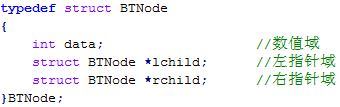
\includegraphics[width=3.54167in,height=1.11458in]{png-jpeg-pics/BEFD7EF20BBECAF465B5B19292AE6ACC.png}
